\part{Introduction}
\chapter{Motivation}
At its origins~\cite{richters:precise:2002,omg:ocl:1997}, \OCL was
conceived as a strict semantics for undefinedness, with the exception
of the logical connectives of type \inlineocl{Boolean} that constitute
a three-valued propositional logic.  Recent versions of the \OCL
standard~\cite{omg:ocl:2006,omg:ocl:2012} added a second exception
element, which is given a non-strict semantics.  Unfortunately, this
extension results in several inconsistencies and contradictions. These
problems are reflected in difficulties to define interpreters,
code-generators, specification animators or theorem provers for \OCL
in a uniform manner and resulting incompatibilities of various
tools. For the \OCL community, this results in the challenge to define
a new formal semantics definition \OCL that could replace the ``Annex
A'' of the \acs{ocl} standard~\cite{omg:ocl:2012}.

In the paper ``Extending \OCL with
Null-References''~\cite{brucker.ea:ocl-null:2009} we explored---based
on mathematical arguments and paper and pencil proofs---a consistent
formal semantics that comprises two exception elements:
\inlineocl{invalid} (``bottom'' in semantics terminology) and
\inlineocl{null} (for ``non-existing element'').

This short paper is based on a formalization
of~\cite{brucker.ea:ocl-null:2009}, called ``Featherweight \OCL,'' in
Isabelle/\acs{hol}~\cite{nipkow.ea:isabelle:2002}.  This formalization
is in its present form merely a semantical study and a proof of
technology than a real tool. It focuses on the formalization of the
key semantical constructions, \ie, the type \inlineocl{Boolean} and
the logic, the type \inlineocl{Integer} and a standard strict operator
library, and the collection type \inlineocl{Set(A)} with quantifiers,
iterators and key operators.


\fixme{to be introduced here somewhere. We need this later.}
 \OCL is composed of
 \begin{inparaenum}[1)]
 \item operators on built-in data structures such as Boolean, Integer or Set(\_),
 \item operators of the user-defined data model such as accessors,
   type casts and tests, and
 \item user-defined, side-effect-free methods.
 \end{inparaenum}


% sane default for proof documents
\parindent 0pt\parskip 0.5ex


\chapter{Background}

\section{Formal Foundation}


\subsection{Isabelle}
Isabelle~\cite{nipkow.ea:isabelle:2002} is a \emph{generic} theorem
prover. New object logics can be introduced by specifying their syntax
and natural deduction inference rules. Among other logics, Isabelle
supports first-order logic, Zermelo-Fraenkel set theory and the
instance for Church's higher-order logic \acs{hol}, which we choose as
basis for \testgen and which is introduced in the subsequent section.

Isabelle's inference rules are based on the built-in meta-level
implication $\_ \Implies \_$ allowing to form constructs like $A_1
\Implies \cdots \Implies A_n \Implies A_{n+1}$, which are viewed as a
\emph{rule} of the form ``from assumptions $A_1$ to $A_n$, infer
conclusion $A_{n+1}$'' and which is written in Isabelle as
\begin{gather}
  \semantics{A_1 ; \ldots; A_n}\Implies A_{n+1}
  \qquad
  \text{or, in mathematical notation,}
  \qquad
  \begin{prooftree}
    A_1 \qquad \cdots \qquad A_n
    \justifies
    A_{n+1}
    \ptmi{.}
  \end{prooftree}
\end{gather}
The built-in meta-level quantification $\Forall x\spot  x$ captures
the usual side-constraints ``$x$ must not occur free in the
assumptions'' for quantifier rules; meta-quantified variables can be
considered as ``fresh'' free variables. Meta-level quantification
leads to a generalization of Horn-clauses of the form:
\begin{gather}
\Forall x_1, \ldots, x_m\spot \semantics{A_1 ; \ldots; A_n}\Implies
A_{n+1}\mi{.}
\end{gather}

Isabelle supports forward- and backward reasoning on rules.  For
backward-reasoning, a \emph{proof-state} can be initialized and
further transformed into others. For example, a proof of $\phi$, using
the Isar~\cite{wenzel:isabelleisar:2002} language, will look as
follows in Isabelle:
\begin{gather}
  \begin{array}{l}
    \Lemma{label} \phi\\
    \quad\apply{case\_tac}\\
    \quad\apply{simp\_all}\\
  \done
  \end{array}
\end{gather}
This proof script instructs Isabelle to prove $\phi$ by case
distinction followed by a simplification of the resulting proof state.
Such a proof state is an implicitly conjoint sequence of generalized
Horn-clauses (called \emph{subgoals}) $\phi_1$, \ldots,$\phi_n$ and a
\emph{goal} $\phi$. Proof states were usually denoted by:
\begin{gather}
\begin{array}{rl}
\pglabel{label}:& \phi \\
 1.& \phi_1 \\
    &\vdots \\
 n.& \phi_n\\
\end{array}
\end{gather}
Subgoals and goals may be extracted from the proof state into theorems
of the form $\semantics{\phi_1 ; \ldots; \phi_n}\Implies \phi$ at any
time; this mechanism helps to generate test theorems.  Further,
Isabelle supports meta-variables (written $\meta{x}, \meta{y},
\ldots$), which can be seen as ``holes in a term'' that can still be
substituted. Meta-variables are instantiated by Isabelle's built-in
higher-order unification.

\subsection{Higher-order logic}
\emph{Higher-order logic}
(\HOL)~\cite{church:types:1940,andrews:introduction:2002} is a
classical logic based on a simple type system.  It provides the usual
logical connectives like $\_ \land \_$, $\_ \implies\_$, $\lnot \_ $
as well as the object-logical quantifiers $\forall x\spot P\ap x$ and
$\exists x\spot P\ap x$; in contrast to first-order logic, quantifiers
may range over arbitrary types, including total functions
$f\ofType\alpha \Rightarrow \beta$. \HOL is centered around
extensional equality $\_ = \_ \ofType \alpha \Rightarrow \alpha
\Rightarrow \text{bool}$.  \HOL is more expressive than first-order
logic, since, \eg, induction schemes can be expressed inside the
logic. Being based on some polymorphically typed $\lambda$-calculus,
\acs{hol} can be viewed as a combination of a programming language
like \acs{sml} or Haskell and a specification language providing
powerful logical quantifiers ranging over elementary and function
types.

Isabelle/\HOL is a logical embedding of \HOL into Isabelle.  The
(original) simple-type system underlying \HOL has been extended by
Hindley-Milner style polymorphism with type-classes similar to
Haskell.  While Isabelle/\HOL is usually seen as proof assistant, we
use it as symbolic computation environment. Implementations on top of
Isabelle/\HOL can re-use existing powerful deduction mechanisms such
as higher-order resolution, tableaux-based reasoners, rewriting
procedures, Presburger arithmetic, and via various integration
mechanisms, also external provers such as Vampire and the
\acs{smt}-solver Z3.

Isabelle/\HOL offers support for a particular methodology to extend
given theories in a logically safe way: A theory-extension is
\emph{conservative} if the extended theory is consistent provided that
the original theory was consistent.  Conservative extensions can be
\emph{constant definitions}, \emph{type definitions}, \emph{datatype
  definitions}, \emph{primitive recursive definitions} and
\emph{wellfounded recursive definitions}.

For instance, the library includes the type constructor $\up{\tau} :=
\isasymbottom ~ | ~ \lift{\_} : \alpha$ that assigns to each type
$\tau$ a type $\up{\tau}$ \emph{disjointly extended} by the
exceptional element $\isasymbottom$\index{undefinedness lifting}. The
function $\drop{\_} : \up{\alpha} \to \alpha$ is the inverse of
$\lift{\_}$ (unspecified for $\isasymbottom$). Partial functions
$\alpha \isasymrightharpoonup \beta$ are defined as functions $\alpha
\isasymRightarrow \up{\beta}$ supporting the usual concepts of domain
($\dom\;\_$) and range ($\ran\;\_$).

As another example of a conservative extension, typed sets were built
in the Isabelle libraries conservatively on top of the kernel of \HOL
as functions to $\HolBoolean$; consequently, the constant definitions
for membership is as follows:\footnote{To increase readability, we use
  a slightly simplified presentation.}
\begin{gather}
  \begin{array}{lrll}
    \types& \alpha \HolSet            &= \alpha \Rightarrow \HolBoolean\\[.5ex]
    \definitionS &\operatorname{Collect}&\ofType (\alpha \Rightarrow
     \HolBoolean) \Rightarrow \HolSet{\alpha}  &\qquad\text{--- set comprehension}\\
    \where &\operatorname{Collect}\ap S      &\equiv S\\[.5ex]
     \definitionS &\operatorname{member}           &\ofType \alpha \Rightarrow
     \alpha \Rightarrow \HolBoolean &\qquad\text{---
       membership test}\\
     \where &\operatorname{member}\ap s\ap S &\equiv S s\\
  \end{array}
\end{gather}
Isabelle's powerful syntax engine is instructed to accept the notation
$\{x \mid P\}$ for $\operatorname{Collect}\ap\lambda x\spot P$ and the
notation $s \in S$ for $\operatorname{member}\ap s\ap S$. As can be
inferred from the example, constant definitions are axioms that
introduce a fresh constant symbol by some closed, non-recursive
expressions; this type of axiom is logically safe since it works
like an abbreviation. The syntactic side conditions of this axiom are
mechanically checked, of course. It is straightforward to express the
usual operations on sets like $\_ \cup \_,
\_\cap\_\ofType\HolSet{\alpha} \Rightarrow \HolSet{\alpha} \Rightarrow
\HolSet{\alpha}$ as conservative extensions, too, while the rules of
typed set theory were derived by proofs from these definitions.

Similarly, a logical compiler is invoked for the following statements introducing
the types option and list:
\begin{gather}
  \begin{array}{lrll}
    \datatype & \HolOption       &= \HolNone \mid \HolSome{\alpha}\\[.5ex]
    \datatype & \HolList{\alpha} &= \operatorname{Nil} \mid
    \operatorname{Cons}\ap a\ap l
  \end{array}
\end{gather}
Here, $[]$ or $a\#l$ are an alternative syntax for $\operatorname{Nil}$
or $\operatorname{Cons}\ap a ~l$; moreover, $[a, b, c]$ is defined as
alternative syntax for $a\#b\#c\#[]$. These (recursive) statements
were internally represented in by internal type and constant
definitions. Besides the \emph{constructors} $\HolNone$, $\HolSome$,
$[]$ and $\operatorname{Cons}$, there is the match operation
\begin{gather}
\HolCase\ap x\ap\HolOf~\HolNone \isasymRightarrow F\ap \mid
\HolSome{a} \isasymRightarrow G\ap a
\end{gather}
respectively
\begin{gather}
\HolCase\ap x\ap\HolOf~[] \isasymRightarrow F\ap \mid \operatorname{Cons}\ap a\ap
r \isasymRightarrow G\ap a\ap r\mi{.}
\end{gather}
From the internal definitions (not shown here) a number of properties
were automatically derived. We show only the case for lists:
\begin{gather}\label{eq:datatype-rules}
  \begin{array}{ll}
    (\HolCase\ap[]\ap\HolOf\ap[] \Rightarrow F  \ap | \ap  (a\#r) \Rightarrow
    G\ap a\ap r) = F &\\
    (\HolCase \ap  b\#t  \ap \HolOf  \ap [] \Rightarrow F  \ap  | \ap
    (a\#r) \Rightarrow G\ap a\ap r) = G~b~t &\\ %
    \mbox{}[] \neq a\#t    &\text{-- distinctness} \\
    \semantics{ a = [] \implies P ; \exists~x~t\spot  a = x\#t \implies P } \Longrightarrow P &\text{-- exhaust} \\
    \semantics{ P [] ; \forall~at\spot  P t \implies P (a\#t) } \Longrightarrow P x      &\text{-- induct}
  \end{array}
\end{gather}
Finally, there is a compiler for primitive and wellfounded recursive
function definitions. For example, we may define the
$\operatorname{sort}$ operation of our running test example by:
\begin{gather}\label{eq:sortdef}
  \begin{array}{lll}
    \fun
    &\enspace\operatorname{ins} & \ofType
    [\alpha\ofType\mathrm{linorder}, \HolList{\alpha}]
    \Rightarrow
    \HolList{\alpha}\\
    \where
    &\enspace \operatorname{ins}\ap x \ap  [\;] &= [x]\\
    &\enspace \operatorname{ins}\ap x \ap (y\#\mathit{ys})&=
    \HolIf x < y
    \HolThen x\#  y \# ys
    \HolElse y\#(\operatorname{ins} \ap x \ap ys)
 \end{array}\\
  \begin{array}{lll}
    \fun
    &\enspace\operatorname{sort} & \ofType
    \HolList{(\alpha\ofType\mathrm{linorder})}
    \Rightarrow
    \HolList{\alpha}\\
    \where
    &\enspace \operatorname{sort}\ap [\;] &= [\;]\\
    &\enspace \operatorname{sort} (x\#\mathit{xs})&=
    \operatorname{ins}\ap x\ap (\operatorname{sort}\ap xs)
   \end{array}
\end{gather}
The internal (non-recursive) constant definition for these operations
is quite involved; however, the logical compiler will finally derive
all the equations in the statements above from this definition and
make them available for automated simplification.

Thus, Isabelle/\HOL also provides a large collection of theories like
sets, lists, multisets, orderings, and various arithmetic theories
which only contain rules derived from conservative definitions. In
particular, Isabelle manages a set of \emph{executable types and
  operators}, \ie, types and operators for which a compilation to
\acs{sml}, OCaml or Haskell is possible. Setups for arithmetic types
such as $\text{int}$ have been done; moreover any datatype and any
recursive function were included in this executable set (providing
that they only consist of executable operators). Similarly, Isabelle
manages a large set of (higher-order) rewrite rules into which
recursive function definitions were included. Provided that this
rule set represents a terminating and confluent rewrite system, the
Isabelle simplifier provides also a highly potent decision procedure
for many fragments of theories underlying the constraints to be
processed when constructing test theorems.







% \subsection{Higher-order Logic and Isabelle}\label{sec:higher-order-logic}
% Higher-order Logic
% (\acs{hol})~\cite{church:types:1940,andrews:introduction:2002} is a
% classical logic with equality enriched by total polymorphic
% higher-order functions. It is more expressive than first-order logic,
% \eg, induction schemes can be expressed inside the
% logic. Pragmatically, \HOL can be viewed as ``Haskell with
% Quantifiers.''

% \HOL is based on the typed $\lambda$-calculus, \ie, the \emph{terms} of \HOL are
% $\lambda$-expressions.  Types of terms may be built from \emph{type
%   variables}\index{type variables} (like $\alpha$, $\beta$, \ldots, optionally
% annotated by Haskell-like \emph{type classes}\index{type class} as in
% $\alpha::order$ or $\alpha::\Bot$) or \emph{type constructors}\index{type
%   constructor}. Type constructors may have arguments (as in $\HolList{\alpha}$
% or $\HolSet{\alpha}$). The type constructor for the function space
% $\isasymRightarrow$ is written infix: $\alpha \isasymRightarrow \beta$; multiple
% applications like
% $\tau_1\isasymRightarrow(\ldots\isasymRightarrow(\tau_n\isasymRightarrow\tau_{n+1})\ldots)$
% have the alternative syntax $[\tau_1, \ldots, \tau_n] \isasymRightarrow
% \tau_{n+1}$. \HOL is centered around the extensional logical equality $\_=\_$
% with type $[\alpha, \alpha] \isasymRightarrow \HolBoolean$, where $\HolBoolean$
% is the fundamental logical type.  We use infix notation: instead of
% $(\_=\_)~E_1~E_2$ we write $E_1=E_2$. The logical connectives $\_\isasymand\_$,
% $\_\isasymor\_$, $\_\to\_$ of \HOL have type $[\HolBoolean, \HolBoolean]
% \isasymRightarrow \HolBoolean$, $\isasymnot\_$ has type $\HolBoolean
% \isasymRightarrow \HolBoolean$. The quantifiers $\isasymforall\_.\_$ and
% $\isasymexists\_.\_$ have type $[\alpha \isasymRightarrow \HolBoolean]
% \isasymRightarrow \HolBoolean$. The quantifiers may range over types of higher
% order, \ie, functions or sets.
% The definition of the element-hood $\_\isasymin\_$, the set comprehension
% $\{\_.\_\}$, as well as $\_\isasymunion\_$ and $\_\isasyminter\_$ are standard.

% Isabelle is a theorem is generic interactive theorem proving system;
% Isabelle/\HOL is an instance of the former with \HOL.  The
% Isabelle/\HOL library contains formal definitions and theorems for a
% wide range of mathematical concepts used in computer science,
% including typed set theory, well-founded recursion theory, number
% theory and theories for data-structures like Cartesian products
% $\alpha \times \beta$ and disjoint type sums $\alpha + \beta$.
% The library also includes the type constructor $\up{\tau} := \isasymbottom
% ~ | ~ \lift{\_} : \alpha$ that assigns to each type $\tau$ a type
% $\up{\tau}$ \emph{disjointly extended} by the exceptional element
% $\isasymbottom$\index{undefinedness lifting}. The function $\drop{\_}
% : \up{\alpha} \to \alpha$ is the inverse of $\lift{\_}$ (unspecified
% for $\isasymbottom$). Partial functions $\alpha \isasymrightharpoonup
% \beta$ are defined as functions $\alpha \isasymRightarrow \up{\beta}$
% supporting the usual concepts of domain ($\dom\;\_$) and range
% ($\ran\;\_$).
% The library is built entirely by logically safe,
% conservative definitions and derived rules.  This methodology is also
% applied to \holocl~\cite{brucker.ea:hol-ocl:2008} and Featherweight
% \OCL.

% For Journal - or long- version
\subsection{Specification Constructs in Isabelle/\HOL}\label{sec:spec-constructs}


\section{Featherweight OCL: Design Goals}
% generated text of all theories
Featherweight \acs{ocl} is a formalization of the core of \acs{ocl}
aiming at formally investigating the relationship between the
different notions of ``undefinedness,'' \ie, \inlineocl{invalid} and

\inlineocl{null}. As such, it does not attempt to define the complete
\acs{ocl} library. Instead, it concentrates on the core concepts of
\acs{ocl} as well as the types \inlineocl{Boolean},
\inlineocl{Integer}, and typed sets (\inlineocl|Set(T)|).  Following
the tradition of
\holocl~\cite{brucker.ea:hol-ocl:2008,brucker.ea:hol-ocl-book:2006},
Featherweight \OCL is based on the following principles:
\begin{compactenum}
\item It is an embedding into a powerful semantic meta-language and
  environment, namely
  Isabelle/\acs{hol}~\cite{nipkow.ea:isabelle:2002}.
\item It is a \emph{shallow embedding} in \acs{hol}; types
  in \OCL were injectively mapped to types in Featherweight
  \OCL. Ill-typed \OCL specifications cannot be represented in
  Featherweight \OCL and a type in Featherweight \OCL contains exactly
  the values that are possible in \OCL. Thus, sets may contain
  \inlineocl{null} (\inlineocl|Set{null}| is a defined set) but not
  \inlineocl{invalid} (\inlineocl|Set{invalid}| is just
  \inlineocl{invalid}).
\item Any Featherweight \OCL type contains at least
  \inlineocl{invalid} and \inlineocl{null} (the type \inlineocl{Void}
  contains only these instances). The logic is consequently
  four-valued, and there is a \inlineocl{null}-element in the type
  \inlineocl{Set(A)}.
\item It is a strongly typed language in the Hindley-Milner tradition.
  We assume that a pre-process eliminates all implicit conversions due
  to subtyping by introducing explicit casts (\eg,
  \inlineocl{oclAsType()}). The details of such a pre-processing are
  described in~\cite{brucker:interactive:2007}.  Casts are semantic
  functions, typically injections, that may convert data between the
  different Featherweight \OCL types.
\item All objects are represented in an object universe in the \holocl
  tradition~\cite{brucker.ea:extensible:2008-b}. The universe
  construction also gives semantics to type casts, dynamic type
  tests, as well as functions such as \inlineocl{oclAllInstances()},
  or \inlineocl{oclIsNew()}.
\item Featherweight \OCL types may be arbitrarily nested:
  \inlineocl|Set{Set{1,2}} = Set{Set{2,1}}| is legal and true.
\item For demonstration purposes, the set type in Featherweight \OCL
  may be infinite, allowing infinite quantification and a constant
  that contains the set of all Integers.  Arithmetic laws like
  commutativity may therefore be expressed in \OCL itself.  The
  iterator is only defined on finite sets.
\item It supports equational reasoning and congruence reasoning, but
  this requires a differentiation of the different equalities like
  strict equality, strong equality, meta-equality (\acs{hol}). Strict
  equality and strong equality require a subcalculus, ``cp'' (a
  detailed discussion of the different equalities as well as the
  subcalculus ``cp''---for three-valued \acs{ocl} 2.0---is given
  in~\cite{brucker.ea:semantics:2009}), which is nasty but can be
  hidden from the user inside tools.
\end{compactenum}

\section{The Theory Organization}
The semantic theory is organized in a quite conventional manner in
three layers. The first layer, called the \emph{denotational
  semantics} comprises a set of definitions of the operators of the
language.  Presented as \emph{definitional axioms} inside
Isabelle/\HOL, this part assures the logically consistency of the
overall construction. The second layer, called \emph{logical layer},
is derived from the former and centered around the notion of validity
of an \OCL formula $P$ for a state-transition from pre-state $\sigma$
to post-state $\sigma'$, validity statements were written $(\sigma,
\sigma') \models P$.  The third layer, called \emph{algebraic layer},
also derived from the former layers, tries to establish a number of
algebraic laws of the form $P = P'$; such laws are amenable to
equational reasoning and also help for automated reasoning and
code-generation.

For space reasons, we will restrict ourselves in this paper to a few
operators and make a traversal through all three layers in order to
give a high-level description of our formalization.  Especially, the
details of the semantic construction for sets and the handling of
objects and object universes were excluded from a presentation here.

\subsection{Denotational Semantics}
 \OCL is composed of
 \begin{inparaenum}[1)]
 \item operators on built-in data structures such as Boolean, Integer or Set(A),
 \item operators of the user-defined data-model such as accessors,
   type-casts and tests, and
 \item user-defined, side-effect-free methods.
 \end{inparaenum}
 Conceptually, an \OCL expression in general and Boolean expressions in
 particular (\ie, \emph{formulae}) that depends on the pair $(\sigma,
 \sigma')$ of pre-and post-state.  The precise form of states is
 irrelevant for this paper (compare~\cite{brucker.ea:ocl-null:2009})
 and will be left abstract in this presentation. We construct in
 Isabelle a type-class $\TCnull$ that contains two distinguishable
 elements $\HolBot$ and $\HolNull$. Any type of the form
 $\up{(\up{\alpha})}$ is an instance of this type-class with $\HolBot
 \equiv \isasymbottom$ and $\HolNull \equiv \lift{\isasymbottom}$.
 %\fixme{we need this para. bu}
Now, any \OCL type can be represented by an \HOL type of the form:
\begin{equation*}
  \V{}{\alpha} \defeq \state{} \times \state{} \to \alpha \ofType \TCnull \mi{.}
\end{equation*}
On this basis, we define $\V{}{\up{(\up{\HolBoolean })}}$ as the \HOL
type for the \OCL type $\mocl{Boolean}$ by and define:
\begin{gather*}
\begin{alignedat}{3}
I\semantics{\mocl{invalid}\ofType V(\alpha)} \tau &\equiv \HolBot &
I\semantics{\mocl{null}\ofType V(\alpha)}  \tau    &\equiv \HolNull\\
I\semantics{\mocl{true}\ofType\mocl{Boolean}} \tau &=\lfloor\lfloor
\HolTrue\rfloor\rfloor &
I\semantics{\mocl{false}} \tau &= \lfloor\lfloor\HolFalse\rfloor\rfloor\\
\end{alignedat}
\end{gather*}\vspace{-.5cm}
\begin{multline*}
I\semantics{X\mocl{.oclIsUndefined()}} \tau =\\
    (\HolIf I\semantics{X}\tau \in \{\HolBot, \HolNull\} \HolThen I\semantics{\mocl{true}}\tau \HolElse I\semantics{\mocl{false}}\tau)\\
\end{multline*}\vspace{-1.2cm}
\begin{multline*}
 I\semantics{X\mocl{.oclIsInvalid()}} \tau =\\
    (\HolIf I\semantics{X}\tau = \HolBot \HolThen I\semantics{\mocl{true}}\tau \HolElse I\semantics{\mocl{false}}\tau)
\end{multline*}
where $I\semantics{E}$ is the semantic interpretation function
commonly used in mathematical textbooks and $\tau$ stands for pairs of
pre- and post state $(\sigma, \sigma')$. Due to the used style of
semantic representation (a shallow embedding) $I$ is in fact
superfluous and defined semantically as the identity; in Isabelle
theories, it is usually left out in definitions to pave the way for
Isabelle to checks that the underlying equations are axiomatic
definitions and therefore logically safe. For reasons of conciseness,
we will write $\delta~X$ for $\mocl{not}\;X\mocl{.oclIsUndefined()}$
and $\upsilon~X$ for $\mocl{not}\;X\mocl{.oclIsInvalid()}$ throughout
this paper.


On this basis, one can define the core logical operators $\mocl{not}$
and $\mocl{and}$ as follows:
\begin{gather*}
  \begin{array}{ll}
    I\semantics{\mocl{not}\; X}  \tau
    &=  (\HolCase I\semantics{X} \tau  \HolOf\\
    &\quad\begin{array}{ll}
                     ~ \bottom                    &\Rightarrow  \bottom \\
                     | \lfloor  \bottom  \rfloor  &\Rightarrow  \lfloor  \bottom  \rfloor  \\
                     | \lfloor \lfloor  x \rfloor \rfloor  &\Rightarrow  \lfloor \lfloor  \lnot  x \rfloor \rfloor )\\
                   \end{array}\\
   I\semantics{X\;\mocl{and}\; Y}  \tau
    &=  (\HolCase I\semantics{X} \tau  \HolOf\\
    &\quad\begin{array}{ll}
      ~ \bottom                    &\Rightarrow
      (\HolCase I\semantics{Y} \tau  \HolOf\\
      &\quad\begin{array}{ll}
                     ~ \bottom                    &\Rightarrow  \bottom \\
                     | \lfloor  \bottom  \rfloor  &\Rightarrow  \bottom  \\
                     | \lfloor \lfloor  \HolTrue \rfloor \rfloor
                     &\Rightarrow  \bottom\\
                     | \lfloor \lfloor  \HolFalse \rfloor \rfloor
                     &\Rightarrow  \lfloor \lfloor  \HolFalse \rfloor \rfloor )\\
                   \end{array}
      \\
                     | \lfloor  \bottom  \rfloor  &\Rightarrow
      (\HolCase I\semantics{Y} \tau  \HolOf\\
      &\quad\begin{array}{ll}
                     ~ \bottom                    &\Rightarrow
                     \bottom \\
                     | \lfloor  \bottom  \rfloor  &\Rightarrow  \lfloor
                     \bottom \rfloor \\
                     | \lfloor \lfloor  \HolTrue \rfloor \rfloor
                     &\Rightarrow  \lfloor \bottom\rfloor\\
                     | \lfloor \lfloor  \HolFalse \rfloor \rfloor
                     &\Rightarrow  \lfloor \lfloor  \HolFalse \rfloor \rfloor )\\
                   \end{array}
      \\
                     | \lfloor \lfloor  \HolTrue \rfloor \rfloor  &\Rightarrow
      (\HolCase I\semantics{Y} \tau  \HolOf\\
      &\quad\begin{array}{ll}
                     ~ \bottom                    &\Rightarrow
                     \bottom \\
                     | \lfloor  \bottom  \rfloor  &\Rightarrow  \lfloor
                     \bottom \rfloor \\
                     | \lfloor \lfloor y \rfloor \rfloor
                     &\Rightarrow  \lfloor \lfloor  y \rfloor \rfloor )\\
                   \end{array}
      \\
                     | \lfloor \lfloor  \HolFalse \rfloor \rfloor
                     &\Rightarrow   \lfloor \lfloor  \HolFalse \rfloor
                     \rfloor )\\
                   \end{array}\\
  \end{array}
\end{gather*}
These non-strict operations were used to define the other logical connectives in the
usual classical way: $X\; \mocl{or}\; Y \equiv (\mocl{not}\; X)\;
\mocl{and}\; (\mocl{not}\; Y)$ or
$X\;\mocl{implies}\;Y \equiv (\mocl{not}\; X)\;\mocl{or}\; Y$.

The default semantics for an \OCL library operator is strict
semantics; this means that the result of an operation $f$ is
\inlineisar+invalid+ if one of its arguments is \inlineisar+invalid+.
For a semantics comprising \inlineisar+null+, we suggest to stay
conform to the standard and define the addition for integers as
follows:
 \begin{gather*}
   \begin{array}{rl}
   I\semantics{x \mocl{+} y}\tau  = &\HolIf I\semantics{\delta ~ x}\tau =\lfloor \lfloor \HolTrue\rfloor \rfloor  \land   I\semantics{\delta  ~ y}\tau =\lfloor \lfloor \HolTrue\rfloor \rfloor \\
                &\HolThen \lfloor \lfloor \lceil \lceil I\semantics{x}\tau \rceil \rceil  + \lceil \lceil I\semantics{y}\tau \rceil \rceil \rfloor \rfloor\\
                &\HolElse \bottom
   \end{array}
 \end{gather*}
 where the operator ``\mocl{+}'' on the left-hand
 side of the equation denotes the \OCL addition of type
 $[\V{}{\up{(\up{\HolInteger})}}, \V{}{\up{(\up{\HolInteger})}}] \Rightarrow
 \V{}{\up{(\up{\HolInteger})}}$ while the ``$+$'' on the right-hand side of
 the equation of type $[\HolInteger,\HolInteger]\Rightarrow
 \HolInteger$ denotes the integer-addition from the \HOL library.

\subsection{Logical Layer}
The topmost goal of the logic for \OCL is to define the \emph{validity statement}:
\begin{equation*}
   (\sigma, \sigma') \isasymMathOclValid P\mi{,}
\end{equation*}
where $\sigma$ is the pre-state and $\sigma'$ the post-state of the
underlying system and $P$ is a formula.
Informally, a formula $P$ is valid if and only if its evaluation in
$(\sigma, \sigma')$ (\ie, $\tau$ for short) yields true. Formally this means:
\begin{equation*}
\tau \isasymMathOclValid P \equiv \bigl(I\semantics{P} \tau =  \lfloor \lfloor \HolTrue  \rfloor \rfloor \bigr)\mi{.}
\end{equation*}
On this basis, classical, two-valued inference rules can be established for
reasoning over the logical connective, the different notions of equality,
definedness and validity. Generally speaking, rules over logical validity can
relate bits and pieces in various \OCL terms and allow---via strong
logical equality discussed below---the replacement
of semantically equivalent sub-expressions. The core inference rules are:
\begin{gather*}
  \begin{array}{lccr}
  \tau \models \mocl{true}&
  \lnot(\tau \models \mocl{false})&
  \lnot(\tau \models \mocl{invalid})&
  \lnot(\tau \models \mocl{null})
\end{array}\\
  \tau \models \mocl{not}\; P \Longrightarrow \tau \lnot \models P\\
\begin{array}{lcr}
  \tau \models P \;\mocl{and}\; Q \Longrightarrow \tau \models P&\quad&
  \tau \models P \;\mocl{and}\; Q \Longrightarrow \tau \models Q
  \end{array}\\
  \tau \models P \Longrightarrow
     (\mocl{if}\; P \;\mocl{then}\; B_1 \;\mocl{else}\; B_2 \;\mocl{endif})\tau = B_1 \tau\\
  \tau \models \mocl{not}\; P \Longrightarrow
       (\mocl{if}\; P \;\mocl{then}\; B_1 \;\mocl{else}\; B_2 \;\mocl{endif})\tau = B_2 \tau\\
       \begin{array}[lcr]{lcr}
  \tau \models P \Longrightarrow \tau \models \delta P &\qquad&
  \tau \models (\delta X) \Longrightarrow \tau \models \upsilon X
       \end{array}
\end{gather*}
By the latter two properties it can be inferred that any valid
property $P$ (so for example: a valid invariant) is actually defined,
which allows to infer for terms composed by strict operations that
their arguments and finally the variables occurring in it are valid or
defined.

We propose to distinguish the \emph{strong logical equality} (written
$\_ \isasymMathOclStrongEq \_$), which follows the general principle
that ``equals can be replaced by equals,'' from the \emph{strict
  referential equality} (written $\_ \isasymMathOclStrictEq \_$),
which is an object-oriented concept that attempts to approximate and
to implement the former.  Strict referential equality, which is the
default in the \OCL language and is written simply \inlineocl|_ = _|
in the standard, is an overloaded concept and has to be defined for
each \OCL type individually; for objects resulting from class
definitions, it is implemented by simply comparing the references to
the objects. In contrast, strong logical equality is a polymorphic
concept which is defined once and for all by:
\begin{gather*}
  I\semantics{X \triangleq  Y}  \tau  \equiv  \lfloor \lfloor
  I\semantics{X}  \tau=
  I\semantics{Y} \tau  \rfloor \rfloor
\shortintertext{It enjoys nearly the laws of a congruence:}
\tau \models (x \triangleq x)\\
\tau \models (x \triangleq y) \Longrightarrow \tau \models (y \triangleq x)\\
\tau \models (x \triangleq y) \Longrightarrow \tau \models (y \triangleq z) \Longrightarrow \tau \models (x \triangleq z)\\
\HolOclCp P \Longrightarrow \tau \models (x \triangleq y) \Longrightarrow \tau \models (P\ap x) \Longrightarrow \tau \models (P\ap y)
\end{gather*}
where the predicate $\HolOclCp$ stands for \emph{context-passing}, a
property that is characterized by $P(X)$ equals $\lambda \tau\spot
P(\lambda \_\spot X \tau) \tau$. It means that the state tuple $\tau =
(\sigma, \sigma')$ is passed unchanged from surrounding expressions to
sub-expressions. it is true for all pure \OCL expressions (but not
arbitrary mixtures of \OCL and \HOL) in Featherweight \OCL.  The
necessary side-calculus for establishing $\HolOclCp$ can be fully
automated.

The logical layer of the Featherweight \OCL rules gives also a means
to convert an \OCL formula living in its for-valued world into a
representation that is classically two-valued and can be processed by
standard \acs{smt} solvers such as
\acs{cvc3}~\cite{barrett.ea:cvc3:2007} or
Z3~\cite{moura.ea:z3:2008}. $\delta$-closure rules for all logical
connectives have the following format, \eg:
\begin{gather*}
\tau \models \delta x \Longrightarrow (\tau \models \ap\mocl{not}\ap x) = (\lnot (\tau \models x))\\
\tau \models \delta x \Longrightarrow \tau \models \delta y \Longrightarrow (\tau \models x \ap\mocl{and}\ap y) = ( \tau \models x \land \tau \models y)\\
\begin{multlined}
\tau \models \delta x \Longrightarrow  \tau \models \delta y \\
\Longrightarrow (\tau \models (x \ap\mocl{implies}\ap y)) = ( (\tau \models x) \longrightarrow (\tau \models y))
\end{multlined}
\end{gather*}
Together with the general case-distinction
\begin{gather*}
    \tau \models \delta x \lor \tau \models x \triangleq \mocl{invalid} \lor \tau \models x \triangleq \mocl{null} \mi{,}
\end{gather*}
which is possible for any \OCL type, a case distinction on the variables in a formula can be performed; due
to strictness rules, formulae
containing somewhere a variable $x$ that is known to be
$\mocl{invalid}$ or $\mocl{null}$ reduce usually quickly to
contradictions.  For example, we can infer from an invariant $\tau
\models x \isasymMathOclStrictEq y \mocl{-} 3$ that we have actually
$\tau \models x \isasymMathOclStrictEq y \mocl{-} 3 \land \tau \models
\delta x \land \tau \models \delta y$.  We call the latter formula the
$\delta$-closure of the former.  Now, we can convert a formula like
$\tau \models x \mocl{>} 0 ~\text{or} 3 \mocl{*} y \mocl{>} x\mocl{*}x$ into
the equivalent formula $\tau \models x > 0 \lor \tau \models 3
\mocl{*} y \mocl{>} x\mocl{*}x$ and thus internalize the \OCL-logic
into a classical (and more tool-conform) logic. This works---for the
price of a potential, but due to the usually ``rich'' $\delta$-closures
of invariants rare---exponential blow-up of the formula for all \OCL
formulas.

\subsection{Algebraic Layer}
Based on the logical layer, we build a system with simpler rules which
are amenable to automated reasoning. We restrict ourselves to pure
equations on \OCL expressions, where the used equality is the
meta-(\HOL-)equality.

Our denotational definitions on \inlineocl+not+ and \inlineocl+and+
can be re-formulated in the following ground equations:
\begin{gather*}
  \begin{aligned}
  \upsilon\; \mocl{invalid} &= \mocl{false}&
  \upsilon\; \mocl{null} &= \mocl{true}\\
  \upsilon\; \mocl{true} &= \mocl{true}&
  \upsilon\; \mocl{false} &= \mocl{true}\\
\end{aligned}\\[.04\baselineskip]
\begin{aligned}
  %
  \delta\; \mocl{invalid} &= \mocl{false}&
  \delta\; \mocl{null} &= \mocl{false}\\
  \delta\; \mocl{true} &= \mocl{true}&
  \delta\; \mocl{false} &= \mocl{true}\\
\end{aligned}\\[.04\baselineskip]
\begin{aligned}
  %
  \mocl{not}\; \mocl{invalid} &= \mocl{invalid}&
  \mocl{not}\; \mocl{null} &= \mocl{null}\\
  \mocl{not}\; \mocl{true} &= \mocl{false}&
  \mocl{not}\; \mocl{false} &= \mocl{true}\\
\end{aligned}\\[.04\baselineskip]
\begin{aligned}
  %
  (\mocl{null} \;\mocl{and}\; \mocl{true}) &= \mocl{null}&
  (\mocl{null} \;\mocl{and}\; \mocl{false}) &= \mocl{false}\\
  (\mocl{null} \;\mocl{and}\; \mocl{null}) &= \mocl{null}&
  (\mocl{null} \;\mocl{and}\; \mocl{invalid}) &= \mocl{invalid}\\
\end{aligned}\\[.04\baselineskip]
\begin{aligned}
  %
  (\mocl{false} \;\mocl{and}\; \mocl{true}) &= \mocl{false}&
  (\mocl{false} \;\mocl{and}\; \mocl{false}) &= \mocl{false}\\
  (\mocl{false} \;\mocl{and}\; \mocl{null}) &= \mocl{false}&
  (\mocl{false} \;\mocl{and}\; \mocl{invalid}) &= \mocl{false}\\
\end{aligned}\\[.04\baselineskip]
\begin{aligned}
  %
  (\mocl{true} \;\mocl{and}\; \mocl{true}) &= \mocl{true}&
  (\mocl{true} \;\mocl{and}\; \mocl{false}) &= \mocl{false}\\
  (\mocl{true} \;\mocl{and}\; \mocl{null}) &= \mocl{null}&
  (\mocl{true} \;\mocl{and}\; \mocl{invalid}) &= \mocl{invalid}
\end{aligned}\\[.04\baselineskip]
\begin{aligned}
  (\mocl{invalid} \;\mocl{and}\; \mocl{true}) &= \mocl{invalid} \\
  (\mocl{invalid} \;\mocl{and}\; \mocl{false}) &= \mocl{false}\\
  (\mocl{invalid} \;\mocl{and}\; \mocl{null}) &= \mocl{invalid} \\
  (\mocl{invalid} \;\mocl{and}\; \mocl{invalid}) &= \mocl{invalid}\\
\end{aligned}
\shortintertext{On this core, the structure of a conventional lattice arises:}
  \begin{aligned}
    X \;\mocl{and}\; X &= X        &     X \;\mocl{and}\; Y &= Y \;\mocl{and}\; X
  \end{aligned}\\
  \begin{aligned}
    \mocl{false} \;\mocl{and}\; X &= \mocl{false} &
    X \;\mocl{and}\; \mocl{false} &= \mocl{false}  \\
    \mocl{true} \;\mocl{and}\; X  &= X &
    X \;\mocl{and}\; \mocl{true} &= X
  \end{aligned}\\
  \begin{aligned}
             X \;\mocl{and}\; (Y \;\mocl{and}\; Z) &= X \;\mocl{and}\; Y \;\mocl{and}\; Z
  \end{aligned}
\end{gather*}
as well as the dual equalities for \inlineocl{or} and the De Morgan
rules.  This wealth of algebraic properties makes the understanding of
the logic easier as well as automated analysis possible: it allows
for, for example, computing a \acs{dnf} of invariant systems (by
clever term-rewriting techniques) which are a prerequisite for
$\delta$-closures.

The above equations explain the behavior for the most-important
non-strict operations. The clarification of the exceptional behaviors
is of key-importance for a semantic definition the standard and the
major deviation point from
\holocl~\cite{brucker.ea:hol-ocl:2008,brucker.ea:hol-ocl-book:2006},
to Featherweight \OCL as presented here.  The
standard expresses at many places that most operations are strict,
\ie, enjoy the properties (exemplary for \inlineocl{_ + _}):
\begin{gather*}
  \begin{aligned}
  \mocl{invalid}\;\mocl{+}\; x &= \mocl{invalid}&
  \mocl{x} \;\mocl{+}\; \mocl{invalid} &= \mocl{invalid}\\
  x \;\mocl{+}\; \mocl{null} &= \mocl{invalid}&
  \mocl{null} \;\mocl{+}\; x &= \mocl{invalid}
  \end{aligned}\\
  \mocl{null.asType(}X\mocl{)} = \mocl{invalid}
\shortintertext{besides ``classical'' exceptional behavior:}
  \begin{aligned}
    \mocl{1 / 0} &= \mocl{invalid} \quad &\quad  \mocl{1 / null} &= \mocl{invalid}
  \end{aligned}\\
    \mocl{null->isEmpty()}=\mocl{true}
\end{gather*}

Moreover, there is also the proposal to use \inlineocl+null+ as a kind
of ``don't know'' value for all strict operations, not only in the
semantics of the logical connectives.  Expressed in algebraic
equations, this semantic alternative (this is \emph{not}
Featherweight \OCL at present) would boil down to:
\begin{gather*}
  \begin{aligned}
    \mocl{invalid} \;\mocl{+}\; x &= \mocl{invalid} &
    x \;\mocl{+}\; \mocl{invalid} &= \mocl{invalid}\\
    x \;\mocl{+}\; \mocl{null} &= \mocl{null}&
    \mocl{null} \;\mocl{+}\; x &= \mocl{null}\\
    1 / 0 &= \mocl{invalid}&
    1 / \mocl{null} &= \mocl{null}
  \end{aligned}\\
  \begin{aligned}
    \mocl{null->isEmpty()}&=\mocl{null}&
    \mocl{null.asType(}X\mocl{)} &= \mocl{null}
\end{aligned}
\end{gather*}

While this is logically perfectly possible, while it can be argued
that this semantics is ``intuitive,'' and although we do not expect a
too heavy cost in deduction when computing $\delta$-closures, we
object that there are other, also ``intuitive'' interpretations that
are even more wide-spread: In classical spreadsheet programs, for
example, the semantics tends to interpret \inlineocl+null+
(representing empty cells in a sheet) as the neutral element of the
type, so \inlineocl{0} or the empty string, for example.\footnote{In
  spreadsheet programs the interpretation of \inlineisar+null+ varies
  from operation to operation; \eg, the \inlineocl+average+
  function treats \inlineocl+null+ as non-existing value and not as
  \inlineocl{0}.}  This semantic alternative (this is
\emph{not} Featherweight \OCL at present) would yield:
\begin{gather*}
  \begin{aligned}
    \mocl{invalid} \;\mocl{+}\; x &= \mocl{invalid} &
    x \;\mocl{+}\; \mocl{invalid} &= \mocl{invalid}\\
    x \;\mocl{+}\; \mocl{null} &= x&
    \mocl{null} \;\mocl{+}\; x &= x\\
    1 / 0 &= \mocl{invalid}&
    1 / \mocl{null} &= \mocl{invalid}
  \end{aligned}\\
  \begin{aligned}
    \mocl{null->isEmpty()}&=\mocl{true}&
    \mocl{null.asType(}X\mocl{)} &= \mocl{invalid}
\end{aligned}
\end{gather*}

Algebraic rules are also the key for execution and compilation
of Featherweight \OCL expressions. We derived, \eg:
\begin{gather*}
\delta\; \mocl{Set\{\}} = \mocl{true}\\
\delta\; (X\mocl{->including(}x\mocl{)}) = \delta X \;\mocl{and}\;
\delta x\\
\begin{aligned}
\mocl{Set\{\}->includes(}x\mocl{)} = (\mocl{if}\; \upsilon\; x\; &\mocl{then false}\\
&\mocl{else invalid endif})
\end{aligned}\\
\begin{multlined}
  {(X\mocl{->including(}x\mocl{)->includes(}y\mocl{)})=}\\
  \mbox{\hspace{3.2cm}}\qquad{\begin{aligned}
   (&\mocl{if}\; \delta\; X\\
  &\mocl{then}\;
\begin{array}[t]{l}
\mocl{if}\; x \doteq y\\
\mocl{then true} \\
\mocl{else} X\mocl{->includes(}y\mocl{)}\\
\mocl{endif}
  \end{array}\\
&\mocl{else invalid} \\
         &\mocl{endif})
  \end{aligned}}
\end{multlined}
\end{gather*}
As \inlineocl+Set{1,2}+ is only syntactic sugar for
\begin{ocl}
  Set{}->including(1)->including(2)
\end{ocl}
an expression like \inlineocl+Set{1,2}->includes(null)+ becomes
automatically decidable in Featherweight \OCL by a combination of
rewriting and code-generation and execution. The generated
documentation from the theory files can thus be enriched by numerous
``test-statements'' like:
\begin{isar}[mathescape]
value  "\<tau> \<Turnstile> ($\mathtt{Set\{Set\{2,null\}\}}$ \<doteq> $\;\mathtt{Set\{Set\{null,2\}\}}$)"
\end{isar}
which have been machine-checked and which present a high-level and in
our opinion fairly readable information for \OCL tool manufactures and
users.





\section{A Machine-checked Annex A}
\begin{figure*}[tb]
  \mbox{}\hfill
  \subfloat%
  [The Isabelle jEdit environment. ]%
  {\label{fig:jedit} 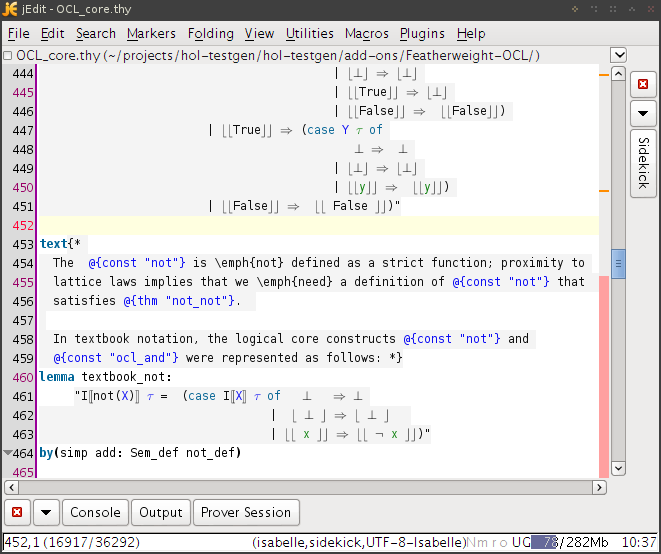
\includegraphics[height=5.5cm]{jedit}}%
  \hfill%
  \hfill%
    \subfloat[The generated formal document.]%
    {\label{fig:pdf} 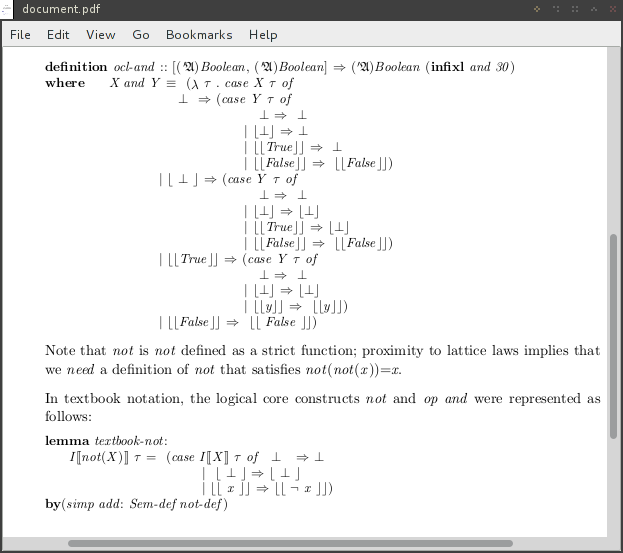
\includegraphics[height=5.5cm]{pdf}}
    \hfill\mbox{}
  \caption{Generating documents with guaranteed  syntactical and
    semantical consistency.}
  \label{fig:gener-docum-where}
\end{figure*}
Isabelle, as a framework for building formal
tools~\cite{wenzel.ea:building:2007}, provides the means for
generating \emph{formal documents}.
With formal documents we refer to documents that are machine-generated
and ensure certain formal guarantees. In particular, all formal
content (\eg, definitions, formulae, types) are checked for
consistency during the document generation.

For writing documents, Isabelle supports the embedding of informal
texts using a \LaTeX-based markup language within the theory files. To
ensure the consistency, Isabelle supports to use, within these
informal texts, \emph{antiquotations} that refer to the formal parts and
that are checked while generating the actual document as
\acs{pdf}. For example, in an informal text, the antiquotation
\inlineisar|@{$\text{thm}$ "not_not"}| will instruct Isabelle to lock-up the
(formally proven) theorem of name \inlineisar"ocl_not_not" and to replace
the antiquotation with the actual theorem, \ie,
\inlineocl{not (not x) $=$ x}.

\autoref{fig:gener-docum-where}
illustrates this approach: \autoref{fig:jedit} shows the jEdit-based
development environment of Isabelle with an excerpt of one of the core
theories of Featherweight \OCL. \autoref{fig:pdf} shows the generated
\acs{pdf} document where all antiquotations are replaced. Moreover,
the document generation tools allows for defining syntactic sugar as
well as skipping technical details of the formalization.


Thus, applying the Featherweight \OCL approach to writing an updated
Annex A that provides a formal semantics of the most fundamental
concepts of \OCL would ensure
\begin{inparaenum}
\item that all formal context is syntactically correct and well-typed,
  and
\item all formal definitions and the derived logical rules are
  semantically consistent.
\end{inparaenum}
